\documentclass[11pt]{article}
\usepackage{amsmath,amssymb,amsthm}
\usepackage[margin=1.1in]{geometry}
\usepackage{booktabs}
\usepackage{tikz}
\usepackage{hyperref}

\newtheorem{definition}{Definition}
\newtheorem{theorem}{Theorem}
\newtheorem{proposition}{Proposition}
\theoremstyle{remark}
\newtheorem{remark}{Remark}

\newcommand{\E}{\mathbb{E}}
\newcommand{\Var}{\operatorname{Var}}

\title{The Multinoulli (Categorical) Distribution}
\author{Yuval Lavie}
\date{\today}

\begin{document}
\maketitle

\begin{abstract}
A self-contained reference for the multinoulli distribution ---
Bernoulli with $K$ outcomes: definition and properties, statistics of
the count estimator, maximum likelihood and maximum a posteriori
estimation under the Dirichlet prior (with full derivations),
information functions, and the numerical solution by stochastic
gradient descent on softmax logits. All quantitative statements are
verified by the companion program \texttt{multinoulli.py}.
\end{abstract}

\section{The distribution}

\begin{definition}
$X \sim \mathrm{Multinoulli}(p_1, \dots, p_K)$, with $p$ in the
simplex ($p_j \ge 0$, $\sum_j p_j = 1$), if $\Pr(X = j) = p_j$ for
$j \in \{1, \dots, K\}$. In one-hot coordinates
$e_X \in \{0,1\}^K$ the pmf is
\begin{equation}
  f(x; p) \;=\; \prod_{j=1}^{K} p_j^{\,\mathbf{1}[x = j]}.
  \label{eq:pmf}
\end{equation}
\end{definition}

\begin{center}
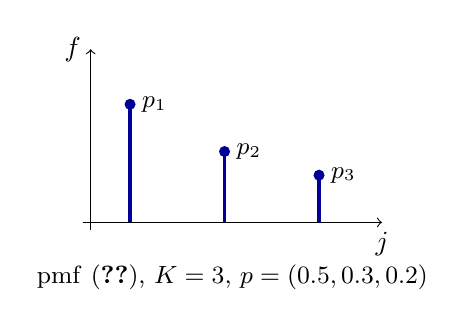
\begin{tikzpicture}[scale=1.0]
\draw[->] (-0.6,0) -- (3.2,0) node[below] {$j$};
\draw[->] (-0.5,-0.1) -- (-0.5,2.2) node[left] {$f$};
\foreach \j/\h/\l in {0/1.5/{p_1}, 1.2/0.9/{p_2}, 2.4/0.6/{p_3}} {
  \draw[very thick,color=blue!60!black] (\j,0) -- (\j,\h);
  \fill[color=blue!60!black] (\j,\h) circle (2pt);
  \node[right] at (\j+0.03,\h) {\small $\l$};
}
\node at (1.3,-0.7) {\small pmf \eqref{eq:pmf}, $K = 3$,
  $p = (0.5, 0.3, 0.2)$};
\end{tikzpicture}
\end{center}

\begin{center}
\begin{tabular}{ll}
\toprule
Support & $\{1, \dots, K\}$ (one-hot: vertices of the simplex)\\
Parameter & $p$ in the $(K{-}1)$-simplex\\
Mean (one-hot) & $\E[e_X] = p$\\
Covariance & $\operatorname{Cov}[e_X] =
  \operatorname{diag}(p) - p\,p^{\!\top}$\\
Mode & $\arg\max_j p_j$\\
Entropy & $-\sum_j p_j \log p_j$\\
Fisher information & $I(p)_{jj} = 1/p_j$ (free coordinates
  $p_1..p_{K-1}$: $\operatorname{diag}(1/p) + \tfrac{1}{p_K}
  \mathbf{1}\mathbf{1}^{\!\top}$)\\
Conjugate prior & $\mathrm{Dirichlet}(\alpha_1, \dots, \alpha_K)$\\
\bottomrule
\end{tabular}
\end{center}

The off-diagonal covariances are \emph{negative},
$\operatorname{Cov}(\mathbf{1}[X{=}i], \mathbf{1}[X{=}j]) =
-p_i p_j$: one category firing forbids the others.

\begin{proposition}[Exponential family form]
With natural parameters $\theta_j = \log(p_j / p_K)$,
$j = 1..K{-}1$, and log-partition
$A(\theta) = \log\bigl(1 + \sum_{j<K} e^{\theta_j}\bigr)$, the pmf is
a full-rank exponential family with sufficient statistic the one-hot
vector; $\partial A/\partial \theta_j = p_j$ recovers the softmax
mean map.
\end{proposition}

\section{Statistics of the estimator}

Let $x_1, \dots, x_n$ be i.i.d.\ with counts
$n_j = \#\{i : x_i = j\}$.

\begin{proposition}[Sufficiency]
$L(p) = \prod_j p_j^{n_j}$: the counts $(n_1, \dots, n_K)$ are
jointly sufficient (factorization), and complete (full-rank
exponential family).
\end{proposition}

\begin{proposition}[Properties of $\hat p_j = n_j / n$]
Each coordinate is a Bernoulli sample mean: unbiased,
$\Var(\hat p_j) = p_j(1 - p_j)/n$ at the Cram\'er--Rao bound,
UMVUE by Lehmann--Scheff\'e, strongly consistent, and jointly
asymptotically normal:
$\sqrt{n}(\hat p - p) \to \mathcal{N}\bigl(0,
\operatorname{diag}(p) - pp^{\!\top}\bigr)$.
\end{proposition}

\section{Maximum likelihood and maximum a posteriori estimation}

\subsection{Maximum likelihood}

\begin{theorem}[MLE]
\label{thm:mle}
The unique maximizer of $\ell(p) = \sum_j n_j \log p_j$ over the
simplex is
\begin{equation}
  \boxed{\;\hat p_j \;=\; \frac{n_j}{n}.\;}
  \label{eq:mle}
\end{equation}
\end{theorem}

\begin{proof}
Maximize the Lagrangian
$\sum_j n_j \log p_j - \lambda(\sum_j p_j - 1)$: stationarity gives
$n_j / p_j = \lambda$ for every $j$, i.e.\ $p_j = n_j/\lambda$;
the constraint forces $\lambda = \sum_j n_j = n$. The objective is
strictly concave on the simplex interior, so the point is the unique
maximum. (Gibbs' inequality provides a second proof:
$\mathrm{NLL}(q) - \mathrm{NLL}(\hat p) = n\,\mathrm{KL}(\hat p\|q)
\ge 0$.)
\end{proof}

\subsection{Maximum a posteriori}

\begin{proposition}[Conjugacy]
Let $p \sim \mathrm{Dirichlet}(\alpha)$, i.e.\
$\pi(p) \propto \prod_j p_j^{\alpha_j - 1}$. Then
\begin{equation*}
  \pi(p \mid x_{1:n}) \;\propto\; \prod_j p_j^{\,n_j + \alpha_j - 1}
  \;=\; \mathrm{Dirichlet}(n_1 + \alpha_1, \dots, n_K + \alpha_K).
\end{equation*}
\end{proposition}

\begin{theorem}[MAP]
For $n_j + \alpha_j > 1$ for all $j$,
\begin{equation}
  \boxed{\;\hat p_j^{\mathrm{MAP}}
  \;=\; \frac{n_j + \alpha_j - 1}{\,n + \sum_k \alpha_k - K\,}.\;}
  \label{eq:map}
\end{equation}
\end{theorem}

\begin{proof}
The log-posterior is, up to a constant,
$\sum_j (n_j + \alpha_j - 1)\log p_j$. Maximizing subject to
$\sum_j p_j = 1$ with a Lagrange multiplier: stationarity gives
$(n_j + \alpha_j - 1)/p_j = \lambda$, so
$p_j = (n_j + \alpha_j - 1)/\lambda$, and summing over $j$ forces
$\lambda = n + \sum_k \alpha_k - K$, which is \eqref{eq:map} ---
Theorem~\ref{thm:mle}'s computation with the prior's pseudo-counts
$\alpha_j - 1$ added to the data's. Concavity gives uniqueness.
\end{proof}

\begin{remark}[Additive smoothing is MAP]
The symmetric prior $\alpha_j = 1 + \alpha$ yields
$\hat p_j = (n_j + \alpha)/(n + K\alpha)$: Laplace/add-$\alpha$
smoothing, used throughout Generative/text-to-text, is exactly MAP
estimation under a symmetric Dirichlet. The flat prior
$\alpha_j = 1$ recovers the MLE; as $n \to \infty$ the prior fades.
\end{remark}

\section{Information theory}

The score in the free coordinates is
$s_j = \mathbf{1}[x{=}j]/p_j - \mathbf{1}[x{=}K]/p_K$, with
$\E[s] = 0$ and covariance the Fisher matrix of the table. Entropy
$H(p) = -\sum_j p_j \log p_j$ is maximal at the uniform distribution
($\log K$); for two multinoullis
\begin{equation}
  \mathrm{KL}(p \,\|\, q) = \sum_j p_j \log\frac{p_j}{q_j} \ge 0,
  \qquad
  H(p, q) = H(p) + \mathrm{KL}(p \| q),
  \label{eq:kl}
\end{equation}
and minimizing the empirical cross-entropy over $q$ is Theorem
\ref{thm:mle} again (Gibbs). The Jeffreys prior is
$\mathrm{Dirichlet}(\tfrac12, \dots, \tfrac12)$.

\section{Numerical solution by stochastic gradient descent}

Parameterize the simplex by logits, $p = \mathrm{softmax}(z)$,
$z \in \mathbb{R}^K$, and minimize the average NLL
$F(z) = -\sum_j \hat p_j \log \mathrm{softmax}(z)_j$.

\begin{proposition}[Gradient]
\begin{equation}
  \boxed{\;\nabla_z F = \mathrm{softmax}(z) - \hat p,
  \qquad
  g_i(z) = \mathrm{softmax}(z) - e_{x_i}.\;}
  \label{eq:grad}
\end{equation}
\end{proposition}

\begin{proof}
With $s = \mathrm{softmax}(z)$,
$\partial \log s_j / \partial z_k = \mathbf{1}[j{=}k] - s_k$
(differentiate $z_j - \log\sum_l e^{z_l}$). Hence
$\partial F/\partial z_k = -\sum_j \hat p_j(\mathbf{1}[j{=}k] - s_k)
= s_k - \hat p_k$, using $\sum_j \hat p_j = 1$. The per-sample case
replaces $\hat p$ by the one-hot $e_{x_i}$; its expectation over a
uniform index restores $\hat p$.
\end{proof}

SGD over shuffled passes descends to a noise ball around the softmax
image of \eqref{eq:mle} (identifiable up to a common logit shift);
the Polyak average of the final pass is reported, and autograd on
\texttt{cross\_entropy} reproduces \eqref{eq:grad} on an identical
schedule.

\section{Numerical verification}

\texttt{multinoulli.py} ($p = (0.5, 0.3, 0.2)$, seed 7):

\begin{center}
\begin{tabular}{lll}
\toprule
Claim & Reference & Measured\\
\midrule
$\E[e_X] = p$,
  $\operatorname{Cov} = \operatorname{diag}(p) - pp^{\!\top}$
  & \S1 & entrywise $< 5\times10^{-3}$\\
MLE beats 500 challengers & Thm.~\ref{thm:mle} & min excess
  $\ge 0$\\
$\mathrm{sd}(\hat p_j)$ vs.\ $\sqrt{p_j(1-p_j)/n}$ & \S2 &
  within a few \%\\
Flat Dirichlet: MAP $=$ MLE & \eqref{eq:map} & exact\\
Add-$\alpha$ smoothing $=$ MAP & Rem.~1 & exact identity\\
Polyak vs.\ count table & \eqref{eq:grad} & within $10^{-2}$\\
Hand SGD vs.\ autograd & \eqref{eq:grad} & max gap $< 10^{-10}$\\
\bottomrule
\end{tabular}
\end{center}

\end{document}
